\section{Analysis}

\subsection{Comparing Measurement Methods}

The methods of collecting data to track IPv6 deployment presented all have
advantages and disadvantages, and the different approaches provide a view of
different facets of the deployment and use of IPv6 on the internet. 

Prefix allocation data gives a complete view of all the addresses allocated by
IANA and the RIRs, with all RIRs publishing the details of which prefixes they
have allocated and to whom they have allocated them to. Unfortunately there is
no way to gain a greater depth than RIR though, so no data is available on how
LIRs such as ISPs are allocating prefixes out their own prefixes. The allocation
data is made easily accessible by all the RIRs, and in particular RIPE NCC make
an effort to make their allocation data accessible and to provide tools to allow
analysis and generation of statistics on the data\cite{ripe_ncc_ripestat_2011}. Historical data for
past allocations is complete by definition as the RIRs must keep complete
records of all the prefix allocations they make to administer allocation. One of
the most important properties of a measurement approach is how well it
represents the state of IPv6 deployment, an area in which prefix allocation data
falls short, as the request for and allocation of prefixes to organisations does
not imply use of that prefix, and Karpilovsky et al. find that a significant
proportion of prefix allocated are never announced via BGP so are not
reachable\cite{karpilovsky_quantifying_2009}.
However, the data still reveals underlying trends in the deployment of IPv6 as
the proportion of LIRs that request address space and then advertise a route to
that prefix remains fairly static.

Routing data detailing the BGP routes announced by ASs across the internet
provides a good view of how IPv6 is supported on the backbone of the internet,
and the total amount of address space being advertised, but lacks data from the
edge of the internet. The BGP tables also vary depending on where the data is
collected from, as different nodes on the internet have differing view of the
structure of the internet, particularly if route aggregation is taken into
account. A number of projects make BGP routing data freely available, collecting
route information from a number of sources to get a more complete data set. As
BGP routing data is a well established source of data for performing
measurements of internet infrastructure, good historical data is generally
available, supported by both RIRs and IXPs. As a representation of the state of
deployment of IPv6, routing data gives a more accurate account of which IPv6
prefixed are in use, although route aggregation may limit the usefulness of data
in some cases, and even announcing a BGP route for an IPv6 prefix does not
imply that an LIR or any of its customers are providing any services from those
addresses.

Data for the availability of services and usage of those services over IPv6 is
much less complete, in part caused by the de-centralised nature of the internet
meaning that it is very difficult to capture data from all of the content
providers and consumers of the internet. However, it is possible to attain a
reasonably representative sample by looking at the more popular services
available, as the majority of traffic goes to or from these services making it
possible for companies like Google to collect usage data from a very wide user
base, and for service availability data to be collected by iterating through
publicly available lists of the most visited sites on the web. Service
availability data is also more difficult to collect than prefix allocation and
routing data, as it is necessary to actively probe service providers to find if
their services are available over IPv6. Despite the negative aspects of service
availability and usage data, it is a very good indicator of progress of IPv6
transition as the provision and use of services over IPv6 is the definition of
success for IPv6 deployment. Unfortunately most of the efforts to collect this
type of data are relatively recent in comparison to collection of routing and
allocation data, so historical records do not cover as far back as those for
routing and allocation data.

It is also possible to combine some approaches to permit further analysis,
particularly in tracking the how changes in IPv6 deployment progress from
organisations requesting new addresses, to advertising those addresses, to
providing services using those addresses, to users accessing those
services over IPv6.

\subsection{Analysis of IPv6 Deployment}

\subsubsection{Analysing Service Availability Data}

An aspect of service availability data that has not been widely investigated is
the trends in the data over time; Prior does not keep historical data, and no
analysis has yet been performed on the service availability data set collected
by Crépin-Leblond at \verb+ipv6matrix.org+. Data for the IPv6 Matrix is
collected and stored separately for each top level domain (TLD) and each data set
is archived by time of measurement completion. The analysis presented here is
based upon that presented by Crépin-Leblond in
\cite{olivier_mj_crepin-leblond_ipv6_2011}, finding the percentage of hosts
surveyed that support access to web, mail, DNS or NTP using IPv6, shown in
Figure \ref{fig:output} for the .com, .uk, .net, .org, and .de TLDs. The graph shows
similar results to the other data sources, with a sharp increase in number of
IPv6 enabled services in mid-2011. The increases shown in Figure
\ref{fig:output} can almost
certainly be attributed to the success of ``World IPv6 Day'' and ``World IPv6 Launch''
as the largest
increases occur in the first scan completed after the 6th of June 2011 and 6th
June 2012
for each TLD, correlating with the number of content providers that enabled IPv6
for their services on these dates.

\begin{figure}[htb]
\centering
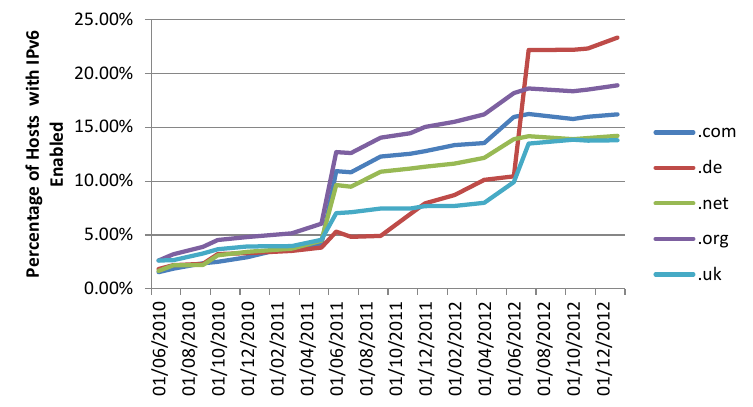
\includegraphics[width=0.45\textwidth]{img/output.png}
\caption{Percentage of Hosts with IPv6 enabled for .com, .uk, .net, .org, and
.uk TLDs}
\label{fig:output}
\end{figure}

\subsubsection{Factors Affecting IPv6 Deployment}

As discussed in the introduction, to ease the challenges faced by organisations
wanting to move away from IPV4 to IPv6, the NGTrans working group was formed by
the IETF to produce recommendations for transition tools and policies. Many
proposals were generated, with some proposals becoming standards, but little
guidance given on how to use the transition mechanisms effectively. The 6to4
tunnelling mechanism designed to allow hosts to connect to IPv6 services over
IPv4 specified in 2001 \cite{rfc3056}, is a good example of a transition mechanism that
has quite possibly hindered deployment of IPv6 rather than helping. 6to4 relies
on a network of anycast relays to interface between the IPv4 and IPv6 internet,
a feature intended to allow automatic tunnel configuration, but which in
practice causes the protocol to be very unstable as not all relays can reach the
entire IPv6 internet and operation of the relays is not regulated. Aben finds
that around 15\% of connections made using 6to4 fail\cite{aben_6to4_2011}, an unacceptable
level for content providers considering switching their services to dual-stack.
Figure \ref{fig:google-access} shows that 6to4 usage has become negligible,
mitigating the stability issues. However, issues such as this one combined with
the large number of transition methods available; Steffann et al.
identifying 16 different mechanisms for tunnelling IPv6 traffic over IPv4
\cite{draft-steffann-tunnels},
contribute to FUD surrounding making the transition to IPv6, as content
providers are unwilling to serve content over IPv6 if this will cause some users
to become unable to access the content.

A major concern for both content providers and ISPs is the performance and
reliability of IPv6 compared to IPv4. In particular, organisations do not want
customers/clients to become unable to access any services that organisation
provides as a result of deploying their services onto IPv6. Colitti et al. find
that the latency of IPv6 connections to google.com is slightly lower than that
of IPv4 connections, despite tunnelling overheads, although Colitti et al. also
state that this may be due to the relatively high proportion of research
institutions using IPv6. Dhamdhere et al. find that IPv6 performance is
comparable where the paths taken across the Internet are identical, but IPv6 may
perform poorly in comparison if the path is longer due to tunnelling or lack of support in
backbone links. This highlights the importance of IPv6 support on Internet
backbone links as shown by the allocation and BGP data.

When conducting analysis on measurement data for IPv6 deployment and attempting
to determine factors that may be affecting the progress of deployment, technical
factors are primarily explored. It is however important not to dismiss the
effect business factors may have on the state of IPv6 deployment. Business
factors that affect content providers include reaching clients that only have
IPv6, something that will become increasingly commonplace due to the exhaustion
of the IPv4 address space, the ability for an organisation to control its own
address space as many organisation may not want to be reliant on their ISP to
provide addressing so PI address space may be viewed as a requirement by these
organisations. Service providers will also consider the possible expense
involved when considering deploying IPv6, although this should not be great in
terms of replacing hardware and software as IPv6 support is widely available in
most modern network hardware and server software. However, there is likely to be
some cost involved in planning the deployment and applying the necessary
configuration changes. ISPs have a slightly different set of business concerns
and must consider how to meet the demand for address space from customers, with
limited options for supplying further IPv4 address space. Expense is a major
factor for ISPs, as deploying a fully IPv6 capable infrastructure may be
prohibitively expensive. Transition tools such as 6rd, a tunnelling mechanism
designed to let an ISP tunnel IPv6 traffic from the edge of their network to the
ISPs IPv6 Point of Presence (POP) over existing IPv4 infrastructure using a
specialisation of the 6to4 protocol, allow ISPs to incrementally upgrade
infrastructure to IPv6, as successfully demonstrated by free.fr(cite). One other
factor an ISP may consider is demand for IPv6 from customers wanting to access
content or serve content using IPv6, a factor absent from many consumer ISPs
where customers do not necessarily care about how content is delivered at the
network layer, only that content delivery works at the application layer. Events
such as World IPv6 Day aim to educate users of the web about why IPv6 is
necessary and how it affects them.

\subsubsection{Combining Measurements}

To build upon the existing analysis performed by Kuhne and Karpilovsky, it is
possible to extend the classification of stages in the life of IPv6 deployment
to the other measurement methods. The experimental phase identified by Kuhne is
unfortunately only visible in the prefix allocation data, as no records
generally exist for the other data collection methods. The period between 2002
and 2007-9 where there was little increase in IPv6 deployment is replicated
across the prefix allocation data and BGP data, with no data existing for usage
and service availability until around 2009. Between 2009 and 2011 both the BGP
and prefix allocation sources indicate rapid growth, although this increase is
not reproduced in the usage and service availability data, with data from Google
only showing slight growth, and IPv6 Matrix data also showing slight growth.
After June 2011 the BGP announcements and prefix allocations drop off slightly,
possibly caused by a rush to support IPv6 running up to World IPv6 Day on the
6th June 2011. Both the Google data and IPv6 Matrix data shows significant
increase in 2012, with the IPv6 Matrix showing a large jump in services
available using IPv6 around the World IPv6 Launch whilst the Google data shows a
more gentle increase throughout the year. It is interesting to note the
difference between the IPv6 support enabled before World IPv6 Day and the change
in service availability around World IPv6 Launch day, where participants'
services had IPv6 enabled permanently rather than just for a day. All of the
measurement methods appear to show IPv6 deployment increasing steadily into the
future.


%Returning to the discussion of the history of deployment of IPv6, it is clear
%that between 1998 when the specification of IPv6 was released and 2008 that the
%transition from IPv4 to IPv6 was much slower than the community had hoped(cite).
%Using the measurements and analysis thereof collected it is possible to propose
%some reasons why this may have been the case. 


%\subsection{Using Measurements to Promote Deployment}

%\item can we use different methods together to get a better picture of IPv6 deployment.
%\item recent changes, the current state of IPv6, what the measurements are currently telling us.
%\item can we in any way make any useful predictions about the future of IPv6 deployment (and has anyone else made reasonable forecasts previously)
%\item spend some time explaining why IPv6 is not currently as deployed as it could be.
